\documentclass[12pt, a4paper]{article}
\setlength{\parindent}{0em}
\setlength{\parskip}{1.4ex}
\usepackage[english]{babel}
\usepackage[utf8]{inputenc}
\usepackage{graphicx}
\usepackage{amsmath}
\usepackage{listings}
\usepackage{textcomp}
\usepackage{xcolor}
\usepackage{fancyhdr}
\definecolor{listinggray}{gray}{0.9}
\definecolor{lbcolor}{rgb}{0.9,0.9,0.9}
\definecolor{backcolour}{rgb}{0.95,0.95,0.92}
\lstdefinestyle{JavaStyle}{
	language=Java,      % choose the language of the code
	deletekeywords={new,public},
	keywords=[2]{HashMap,Map,SimpleDateFormat,String},
	keywords=[3]{getKmaxDevice,getKmaxWidget,getKmaxHist,init},
	basicstyle=\scriptsize\ttfamily,
	keywordstyle=\color[RGB]{69,97,189},
	keywordstyle=[2]{\color{cyan}},
	keywordstyle=[3]\color[RGB]{137,77,155},
	commentstyle=\itshape\color{green!60!black},
	moredelim=[l][\itshape\color{gray}]{//}, %<--- overrides line-comment style
	stringstyle=\color[RGB]{192,8,8},
	numberstyle=\itshape\color{yellow!50!black},
	backgroundcolor=\color{lbcolor},
	tabsize=4,
	%   rulecolor=,
	upquote=true,
	aboveskip={1.5\baselineskip},
	columns=fixed,
	showstringspaces=false,
	extendedchars=false,
	breaklines=true,
	prebreak = \raisebox{0ex}[0ex][0ex]{\ensuremath{\hookleftarrow}},
	frame=single,
	numbers=left,
	showtabs=false,
	showspaces=false,
	showstringspaces=false,
}
\graphicspath{ {images/} }
\pagestyle{fancy}
\fancyhf{}
\rhead{}
\chead{\leftmark}
\lhead{}
\cfoot{\thepage}
\renewcommand{\headrulewidth}{0pt}
\renewcommand{\footrulewidth}{0pt}
\title{Alquerque}
\author{Danny Nicolai Larsen, Mikkel Brix Nielsen \& Steffen Bach}
\date{\today}
\begin{document}
	\maketitle
	\newpage
	\tableofcontents
	\newpage
	\section{Introduction}
	For phase 1 of the project, we have been tasked with implementing the user interface for the board game, Alquerque, by developing a class in accordance with the contract for phase 1. The class has to be executable, meaning it has a main method. The program must start with prompting for the choice of which players are human and which are controlled by the computer. When playing the game, it must prompt the user for a move, and output the moves the computer makes. After each turn it must print the board to the screen. Game continues until a winner is found or there are no valid moves left, resulting in a draw. All the provider classes are precompiled, and thus we should just focus on the interface during this phase.
	
	\section{Design}
	\label{design}
	This section will give an overview of how the program works, and which design choices has been made while writing the program.
	
	\subsection{Option menu \& game initilization}
	The program works by first asking the user to select one of three playable game scenarios; (1) Player vs Player, (2) Player vs CPU, and (3) CPU vs CPU, or (0) to exit the program. The game is then initiated according to what the user picked.
	
	If the user chooses to play against another player, they will be prompted to enter the name of player 1 and then player 2. The game will thereafter commence with player 1 being white and player 2 being black. The game will continue, first prompting the current player, starting with white, to input which piece they want to move followed by where they want to move it, updating the position of the pieces and displaying the updated gamestate to the user, then switching to the next player and repeating the same process for that player. This continues until one of three things happen, either black wins, white wins or the game is a draw. 
	
	Else, if the player chooses to play against a CPU they are first prompted to pick what color they want to play as. The CPU will then play as the opposite color. The player is then prompted to enter their name followed by the number of moves they want the CPU to look ahead while calculating its moves, which determines the level of difficulty. The game will then commence with white making the opening move, may that be either the player or the CPU. Assuming the CPU is white it will calculate its move, in accordance with the number of moves it was allowed to look ahead by the player, and play it. The game state is then updated and displayed, then switching to the player, saying that it is their turn, prompting them to input which piece they want to move followed by where they want to move it. The pieces position are updated and the updated gamestate is displayed, then the CPU makes a move and this cycle continues until either black wins, white wins or the game is a draw. 
	
	Alternatively the user can choose to pit two CPUs against each other, picking how many moves the CPUs are allowed to look ahead, being able to spectate their respective moves as they are calculated and executed. Updating the pieces positions and then displaying them to the user. This continues until either black wins, white wins or the game is a draw.
	
	\subsection{Getters \& setters:}
	Getters and setters have not been implemented because the class is not going to be instantiated, and it is not defined in the contract that another class should be able to use these variables.	
	
	\subsection{Chess notation}
	For improved QOL/user friendliness, we have chosen to assign coordinates to the visual representation of the board with letters, A through E, above and below the board, as well as numbers, 1 through 5, to the left and to the right of the board. Due to the familiarity from chess, this way of identifying board positions should feel more intuitive.
	
	\newpage
	
	\begin{figure}[h]
		\centering
		\caption{Chess Notation}
		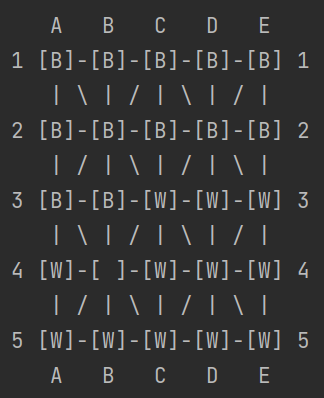
\includegraphics[width=0.4\textwidth]{chessnotation}		
	\end{figure}
	
	\vspace{10mm}
		
	Following this mindset, we decided to represent the board in a two-dimensional array in the size of 6 x 5. The reason we chose this size is that the side of the board which represents the numbers seems more intuitive if the row number corresponds to the rank number on the board, which goes from 1-5. On the other hand the side of the board that represent the letters doesn’t have to correspond in the same way, so we kept the column as going from 0-4
	
	\section{Implementation}
	This section describes the actual technical implementation of the choices described in Section \ref{design}, about design, going in to detail about what methods have been implemented and how they are used.
	
	\subsection{The init() method}
	
	The method init() is the first thing being called when the program starts, when this happens all variables get initialized throughout the method. Firstly the variables which have predefined values get initialized e.g. board becomes a new board, reader becomes a new scanner. Secondly the program greets the user, prints the available options the user can pick from and then prompts the user to pick one of the options, which is then passed through a switch, which is wrapped in a do while loop, which repeats until a valid option is picked. The switch determines which of the available options, if any, the user's input corresponds to. If the user’s input does not correspond to a valid option the switch defaults to telling the users that their inputted option is an invalid option and to try again. This response is followed by the option menu being printed for the user to view the available options again. 
	Depending on which option is chosen, the corresponding variables are defined, and the loop within init() is exited, since a valid option was picked, and the program continues to the main game loop.
	
	\subsection{The main game loop}
	
	In the main game loop the first thing that happens is that the initialized board is presented to the user. After this a check is run determining how the next move should be made. If the next one to play is a player they are prompted to choose a piece corresponding to the color of the player, which turn it is, that they want to move, and then where they want to move the piece, in accordance with standard chess notation. This move is then validated as a valid coordinate. An instance of the move class is then created and passed to isLegal to see if it is a legal move that can be played on the board in the current boardstate. And if that is not the case the user is told that the entered move was invalid and a do-while repeatedly asks the user to input what piece they want to move and where to, until a valid and legal move is entered by the user. While the game is not over this process is repeated switching between black and white. If the player is a CPU, a new move is created in accordance with the calculations done by MiniMaxTree. If the do-while guard, encapsulating the player's moves, registers whether the game is over. An if-statement then checks whether black has won, white has won or if it is a draw between the two. This is then printed to the console for the player to view.
	
	\subsection{Construction of the visual board}
	
	The board is represented in the program by a two-dimensional array, which is constructed in the boardWithPieces() method.
	First it initiates the array, and fills it with empty spaces, defined by the EMPTY constant.
	It then uses the methods black and white from the Board class, to fill in the spaces occupied by black and white pieces.
	\\\\
	
	The printBoard() method, which is used in the main game loop to display the board on the screen, makes an array from boardWithPieces() and prints it out, along with letters from A - B in the top and bottom, numbers from 1-5 in the sides and the guiding lines between the squares.
	
	\subsubsection{Chess notation and functionality}
	
	As mentioned in the design-section, we chose to represent the board with letters for columns and numbers for rows. However, this gives us a String coordinate rather than an integer in the preconditioned range of 1 through 25. So in order to satisfy the precondition for Move, we made the method convertCoordinate that converts an input coordinate to the corresponding positional number, so that it may be used by methods from() and to() in Moved.
	The method works by assigning a numerical value to the coordinate letters, then adding it to a multiplum by 5, which is determined by the coordinate-numbers corresponding array-index.
	\\
	\begin{lstlisting}[style=JavaStyle]
	private static int convertCoordinate(String coord){
		int position = 0;
		switch(Character.toUpperCase(coord.charAt(0))){
			case 'A':   //value of each column is added to the row-determined multiplum of 5 (e.g. D is 4'th, so positional value is +4)
				position = (1+(5*((Integer.parseInt(coord.substring(1))-1))));
				break;
			case 'B':
				position = (2+(5*((Integer.parseInt(coord.substring(1))-1))));
				break;
			case 'C':
				position = (3+(5*((Integer.parseInt(coord.substring(1))-1))));
				break;
			case 'D':
				position = (4+(5*((Integer.parseInt(coord.substring(1))-1))));
				break;
			case 'E':
				position = (5+(5*((Integer.parseInt(coord.substring(1))-1))));
				break;
			default:
				return 0;
		}
		return position;
	}
	\end{lstlisting}
	
	\newpage
	Since the convertCoordinate method has a precondition that it can only accept coordinates that correspond to a number 1-25, we also wrote a method isValidCoords that returns a boolean true/false if the coordinates is a valid place on the board or not. It uses regex to check that it is a two letter string from A1 to E5, which, by the logic used in convertCoordinate, will only translate to numbers between 1 - 25, which therefore satisfies the precondition.

	\begin{lstlisting}[style=JavaStyle]
		private static boolean isValidCoords(String coords){
			return (coords.matches("[A-Ea-e][1-5]")); // Regex for matching
		}
	\end{lstlisting}
	\vspace{10mm}
	For a move to be printed as a coordinate, rather than as the positional integer which the CPU returns when a move is calculated, we had to make a method that would convert Move objects returned from MinMaxTree to the corresponding letters for files and numbers for ranks. The method functions by subtracting 1 from the positional integer, before subtracting 5 until the integer is between 0 and 4, which for each number corresponds to a letter for each file on the board.
	
	To determine the ranks, the positional integer is divided by 5, whereafter 1 is added to compensate for index 0 in the array.
	However, during testing we discovered a minor issue with this method, although, for the most part, it worked as intended, we found the need to subtract 1 from the position before dividing; this will be elaborated in the test section of this report.
	
	\begin{lstlisting}[style=JavaStyle]
    private static String convertPosition(int position){
		String coord = "";
		switch ((position - 1) % 5){
			case 0:
				coord = "A";
				break;
			case 1:
				coord = "B";
				break;
			case 2:
				coord = "C";
				break;
			case 3:
				coord = "D";
				break;
			case 4:
				coord = "E";
				break;
		}
		
		coord = coord + ((position - 1) / 5 + 1);
		return coord;
	}
	\end{lstlisting}
	\vspace{10mm}

	\section{Test}
	This section describes some of the errors and challenges we faced during the construction of the program, either from challenges arising from the calculations, or by limitations of the methods used.
	
	\subsection{Error when inputting non-integers in menus}
	The game crashes when a non-integer input is typed in the menu, or when choosing the cpu depth, as the Scanner method nextInt is used. This causes the program to throw an inputMismatchException.
	
	\subsection{Mistake in B/W input, fixed with regex}
	During testing we found that, when choosing to play white or black, you could type any characters after the B or W and it would still accept it. For example you could write Bwhite, and it would choose black. It was implemented via a switch statement that matched the char at index 0, which of course ignores all other characters following then one at index 0.
	To fix this error, we changed it to an if-else statement, using regex to match B and W specifically, but case insensitive.
	
	\subsection{CPU moves being printed incorrectly}
	When the CPU made a move, we discovered that whenever it was to or from the E file, regardless of rank, the move, although correctly executed, would be printed as a rank 1 higher than intended. An example of this would be the move D1 to E1 being misprinted as “White/Black(CPU) moved D1 to E2”. To fix this, we found that in our method to convert a position represented by an integer to a position represented by a coordinate, we would have to subtract 1 from the position integer before dividing by 5 to get the rank. This meant that position 5 would accurately be converted to 1, instead of 2. The same thing applied to 10, 15, 20, and 25.
	
	\section{Conclusion}
	We didn't encounter a lot of issues in this phase. We went in to the design phase with a clear picture in our minds, which was a movement system, similar to a chess game, with coordinates instead of numbers, and this proved to be a challenge to implement. 
	
	In hindsight this might have made our code a bit more complicated, but we were committed to solving this issue, and implemented several methods to overcome the challenge, without breaching the contract.
	
	We managed to construct a working program without any major issues. The only thing left unsolved is the exception thrown if anything other than an integer is entered when the program expects an integer.
	
	\section{Appendix}
	\subsection{Program Code}
	\lstinputlisting[style=JavaStyle]{../src/Alquerque.java}
\end{document}
